\documentclass[11pt,a4paper,DIV=21,abstract=true,twocolumn]{scrartcl}

\usepackage{booktabs}
\usepackage{url}
\usepackage{xcolor}
\usepackage[colorlinks = true,
            linkcolor = blue,
            urlcolor  = blue,
            citecolor = blue,
            anchorcolor = blue]{hyperref}

\usepackage{multirow}
\usepackage[round, numbers, sort]{natbib}
\usepackage{times}
\usepackage{inputenc}
\usepackage{graphics}
\usepackage{graphicx}
\usepackage[yyyymmdd,hhmmss]{datetime}
\pdfcompresslevel=9
\usepackage{float}
%\usepackage{adjustbox}



\newcommand{\GHI}[1]{\href{https://github.com/EuBIC/EuBIC2023/issues/#1/}{https://github.com/EuBIC/EuBIC2023/issues{#1}}}


\title{Proceedings of the EuBIC-MS Developers Meeting 2023}

\author{
	Pedro Beltrao
\and
Tim Van Den Bossch
\and
Ralf Gabriels
\and
Tanja Holstein
\and
Tobias Kockmann
\and
Alireza Nameni
\and
Christian Panse
\and
Ralph Schlapbach
\and
Ludwig Lautenbacher
\and
Matthias Mattanovich
\and
Alexey Nesvizhskii
\and
Bart Van Puyvelde
\and
Jonas Scheid
\and
Veit Schwämmle
\and
Maximilian Strauss
\and
Anna Klimovskaia Susmelj
\and
Matthew The
\and
Henry Webel
\and
Mathias Wilhelm
\and
Dirk Winkelhardt
\and
Muyao Xi

}

\date{{\small Zürich, Switzerland, \today\ at \currenttime}}

\begin{document}
\maketitle

\begin{abstract}
	The 2023 European Bioinformatics Community for Mass Spectrometry (EuBIC-MS) Developers Meeting was held from January 15th to January 20th, 2023, in Congressi Stefano Franscin at Monte Verità in Ticino, Switzerland. The participants were scientists and developers working in computational mass spectrometry (MS), metabolomics, and proteomics. The 5-day program was split between introductory keynote lectures and parallel hackathon sessions focusing on ``Artificial Intelligence in proteomics'' to stimulate future directions in the MS-driven omics areas. During the latter, the participants developed bioinformatics tools and resources addressing outstanding needs in the community. The hackathons allowed less experienced participants to learn from more advanced computational MS experts and actively contribute to highly relevant research projects. We successfully produced several new tools applicable to the proteomics community by improving data analysis and facilitating future research.


	\vspace{0.5cm}
	\textbf{Keywords:
	}
	Artificial Intelligence,
Benchmark development,
Bioinformatics,
Computational mass spectrometry,
Deep Learning,
Mass spectrometry,
Metabolomics,
Metaproteomics,
Predicted spectra,
Proteomics,
Spectrum clustering,
Visualization

\end{abstract}


\section{Introduction}
The EuBIC-MS Developers Meeting is organized every other year by the European Bioinformatics Community for Mass Spectrometry (EuBIC-MS, eubic-ms.org), an initiative of the European Proteomics Association (EuPA) for user-oriented bioinformatics. EuBIC-MS promotes the use of bioinformatics for mass spectrometry (MS). Our goal is to bring together the European MS bioinformatics community, including students, early-career researchers, and long-standing experts from academia and industry. Through the setup of community-driven initiatives, EuBIC-MS mainly focuses on improving education in computational methods, highlighting job and funding opportunities, promoting international collaborations, publications of specialized studies, and training in specialized software tools. To this end, EuBIC-MS maintains, in collaboration with EuPA, several web resources that include educational videos, grant overviews, a job fair, and tutorials, all available on www.proteomics-academy.org. Besides these online resources, EuBIC-MS regularly organizes workshops and hubs at major international conferences on MS and proteomics. Additionally, an annual conference on computational MS is organized by EuBIC-MS itself, forming an important community outreach effort to bring together bioinformatics researchers from all over Europe.

Since 2017, EuBIC-MS's Winter School takes place every two years \citep{pmid28385664}, (PMID: ?EuBIC2022?). These events are highly attended and are a unique opportunity to learn, discover new tools and methods, and discuss current challenges in the field. However, not all computational expertise is utilized to its full potential in a typical conference setup. Therefore, we alternate the Winter School every other year with a Developers Meeting, which targets software developers and computation-aware end-users. The first official Developers Meeting occurred in Ghent, Belgium, in 2018 \citep{pmid29864591} and Nyborg, Denmark in 2020 \citep{EuBIC-MS2020}. This year's meeting was held at the Congressi Stefano Franscin on Monte Verità in Ticino, Switzerland, from January 15th to January 20th, 2023. A total of 58 participants, including keynote speakers, participated in the meeting (for more statistics see Table 1).  It took off with five keynotes and a poster flash talk session where 26 participants gave a 60-second `elevator pitch' on their poster. In the next four and a half days, the participants split up into seven teams to each work on a project that was proposed and selected through an open call and selection process \href{https://github.com/eubic/EuBIC2023/issues}{eubic/EuBIC2023/issues}. On the final day, we showcased two sponsor presentations and unveiled the output from the hackathons. Additionally, we announced the winner of the best poster. This meeting, organized by and for the European computational MS community, provided a unique opportunity to learn, network, and participate in developing promising tools. The detailed program is available on \url{https://eubic-ms.org/events/2023-developers-meeting}.

\section{Keynote presentations}

\subsection{Alexey Nesvizhskii - Open Search: Open-minded Exploration of Proteomics Data}

Alexey Nesvizhskii  has been fascinated with the subject of the “dark proteome” since his entry in the field proteomics in 2001. What are all those spectra that we cannot identify in a typical search, and how do we design efficient computational strategies to move beyond standard peptide identification searches.  To this end, his group has designed a highly efficient fragment ion indexing algorithm and implemented it in MSFragger \citep{pmid28394336}, which has become a widely used tool and the engine behind our FragPipe computational platform. MSFragger “open” and “mass offset” searches have empowered new strategies for faster and more sensitive identification of biologically or chemically modified peptides. In his presentation, he described recent improvements in their algorithms, including localization-aware open search \citep{pmid32792501} and new methods for the identification of N- and O-linked glycopeptides \citep{pmid33020657}, labile PTMs \citep{pmid37004988}, and chemically labeled peptides in chemoproteomics experiments \citep{pmid37438360}. He  also provided an overview of the various quantification workflows (DIA, TMT, LFQ-MBR) available in FragPipe \url{https://fragpipe.nesvilab.org/}.


\subsection{Maximilian Strauss - Towards the next generation of proteomics analysis with the AlphaPept ecosystem}

Like other omics fields, mass spectrometry (MS)-based proteomics experiences ever-increasing amounts of data with data, demanding swift and effective analysis tools. Tapping into recent computer science strides, we present AlphaPept \citep{Strauss2024}, a Python framework for rapid processing of high-resolution MS data. Utilizing Numba for on-the-fly compilation, AlphaPept offers a hundred-fold increase in processing speed over native Python and can leverage Python's scientific ecosystem and machine learning innovations. Its Jupyter Notebooks facilitate community contributions, while robust engineering practices ensure reliability. AlphaPept can process proteomes within minutes, and supports automated pipelines via a user-friendly interface or use as a library, with its codebase openly available on GitHub. Building on the same design principles, we have since expanded to the AlphaPept ecosystem, which now offers a suite of libraries catering to various stages, from raw data processing to advanced deep learning predictions and downstream statistical and machine learning analyses for biomarker discovery.

\subsection{Mathias Wilhelm - The DOME Recommendations for Machine Learning Exemplified on Prosit}

In light of rising concerns over a reproducibility crisis in machine and deep learning \citep{pmid35883008}, Mathias Wilhelm (Computational Mass Spectrometry, Technical University of Munich, Freising, Germany) presented DOME (data, optimization, model and evaluation), a set of community-wide recommendations for reporting supervised machine learning-based analyses \citep{pmid34316068}, and its interpretation in proteomics research \citep{pmid35119864}. He showed this on the example of developing Prosit, a neural network developed by his group that predicts chromatographic retention time and fragment ion intensities. As machine and deep learning is seeing rapid adoption in proteomics, best practices and reporting standards like DOME are good starting points for scientists, as author and reviewer, to ensure high quality research. The presentation ended by a call to the community: let's learn from each other instead of struggling alone.

\subsection{Anna Susmelj - Predicting physicochemical properties of peptides using deep learning}

Anna Susmelj’s presentation delves into the crucial field of domain generalization in machine learning, with a focus on strategies to bolster model adaptability across diverse datasets while ensuring domain shift robustness. The talk addresses methods to mitigate performance degradation when models confront previously unseen domains, highlighting their practical significance. Additionally, the presentation discusses common pitfalls and testing strategies for AI models in various domains, aiming to contribute to the development of robust and versatile machine learning systems tailored for Mass Spectrometry applications.


\subsection{Pedro Beltrao - Towards a structurally resolved human protein interaction network}

All cellular functions are governed by complex molecular machines that assemble through protein-protein interactions. Their tissue or cell type specificity and atomic details are critical to the study of their molecular and cellular mechanisms but fewer than 5\% of hundreds of thousands of human interactions have been structurally characterized \citep{pmid23399932} and their tissue specificity is essentially unknown. Pedro Beltrao (ETH Zurich) discussed the potential and limitations of recent progress in deep-learning methods using AlphaFold2 to predict structures for human interactions \citep{pmid36690744}. Higher confidence AlphaFold2 models were correctly enriched in interactions supported by affinity purification or structure based methods and can be orthogonally confirmed by spatial constraints defined by cross-link data. In addition, there were several examples of how the predicted binary complexes can be used to build larger assemblies. To study tissue specificity, it was shown how large-scale protein abundance measurements across samples can be used to predict tissue-specific protein interactions \citep{pmid29032074, pmid28854368}. Protein co-variation is a stronger predictor of protein interactions than mRNA co-expression and can be used to build tissue specific protein interaction networks. These tissue specific networks can be used to link trait/disease associated genes to specific tissues and can serve as a resource for studying tissue specific differences in cell biology and disease.



\section{Hackathons}

During the subsequent days, the participants split up into small groups to actively develop bioinformatics applications. Project proposals for the hackathon sessions were crowd-sourced in a transparent and open process \citep{EuBIC2023GitHub} prior to the meeting.
Community members could submit project proposals for hackathon sessions, which were subsequently evaluated on scientific merit and community interest.


\subsection{Maximilian Strauss - DeepScore: Community curated scoring, supercharged with AI}

State of the art for identification in mass-spectrometry-based proteomics is to generate “non-sense”, decoy data and to determine a score cutoff based on a false discovery rate. Nowadays, machine (ML) and deep learning (DL) algorithms are used to learn how to optimally distinguish targets from decoys. While this drastically increases sensitivity, it comes at the cost of explainability, and human-chosen acceptance criteria are replaced with black-box models. This can hinder acceptance in clinical practice, e.g., in peptidomics, where upregulated proteins are investigated by investigating raw data peaks. While other DL-driven domains allow straightforward human validation of the models, e.g., imaging, speech, text, or inspecting a predicted structure from AlphaFold, for proteomics, this is much more challenging. Here, we aim to explore the limitations of the current scoring approach and provide potential solutions. We revisit the idea of confidence by trying to artificially increase identifications with non-sense features, hard decoys, or leaking data. Next, we will build an interactive tool to validate identifications manually and assign human confidence scores. With this, we create a training dataset and build an ML or DL- model to rescore identifications and assign predicted human-level confidence scores (see \citep{issue14}).
%\GHI{14}
%https://github.com/EuBIC/EuBIC2023/issues/14)


\subsection{Matthias Mattanovich and Muyao Xi - MS2 spectra matching for metabolite identification}

One major open topic in untargeted metabolomics is identifying unknown compounds from mass spectra. As MS1 comparisons can be ambiguous (especially for small molecules), we need to look at MS2 spectra, and compare them to public MS2 databases, to differentiate compounds in the same mass range. Currently, the best performing methods for compound identification are GNPS and Sirius. They provide a user with a list of potential compounds, but in some cases the uncertainty is very high or multiple candidates are suggested, making the downstream analysis labor intensive. GNPS improves their predictions by using molecular networks and taking biological information into account[a]. Sirius improves their predictions by comparing structural similarity of the compounds. We would like to set up a novel system, with modular parts that can be tested separately. Each aspect of the pipeline can be improved/modified individually, and multiple methods can be combined as an ensemble. In doing so, this can also serve as a benchmark of existing scoring and matching functions and a testing playground for novel ideas.
During this hackathon \citep{issue13}, different spectral similarity scoring functions were compared and their target and off-target scores were evaluated based on similarity of the compounds.

\subsection{Ludwig Lautenbacher - Shaping a European prediction service for biological data}

We developed Koina (see \url{http://koina.proteomicsdb.org/}), an open-source and modular machine learning (ML) inference server for biological data based on NVIDIA Triton. This platform allows centralizing the hosting of models originating from various training/prediction pipelines such as PyTorch, Sklearn, XGBoost and TensorFlow. Most importantly, models can be accessed by a remote and language-independent interface. A similar system has been used for the last 5 years within Skyline (C\#), the Prosit website (Python), and ProteomicsDB (JavaScript) to access Prosit models. We envision that such a platform will be centrally hosted by, for example, the EBI, and model submission will become a standard practice for publishing new ML models. Although accompanying codebases on platforms like GitHub describe the access of models, they require technical skill to set up. Standardizing the access of the models will dramatically improve reproducibility, and ensure easy access for as many people as possible.
As part of this hackathon \citep{issue12}, we successfully extended our high-performance prediction service, named Koina, by adding multiple machine-learning models from the DeepLC \citep{pmid34711972}, MS2PIP \citep{pmid24078703, pmid25990723}, AlphaPept \citep{pmid36433986} and Prosit \citep{pmid31133760, pmid35549156, pmid34099720} ecosystems. Since then, we have established a common interface between all these models, enabling the seamless generation of predictions with all models \citep{Lautenbacher2024}.
%\GHI{12}


\subsection{Matthew The - Easy-to-use interactive HTML plots collection for data exploration and web tools}

Interactive data exploration and publicly accessible web applications for bioinformatics tools are an essential part of bioinformatics. Ideally, one uses the same framework for both to reduce development time. Shiny apps are popular for this purpose, but are limited to the R language, while Python’s interactive plotting solutions (Plotly, Bokeh) tend to have a steep learning curve and are tricky to deploy. For ProteomicsDB \url{https://www.proteomicsdb.org/}, we developed over a dozen interactive, general-purpose plots based on D3.js and Vue.js \url{https://github.com/wilhelm-lab/proteomicsdb-components}. These range from simple scatter and bar plots to interaction graphs, heatmaps and pathway viewers. We managed to easily reuse and adapt these components in ongoing projects, allowing quick deployment upon publication.For the hackathon, we propose releasing these plots as Web Components \url{https://www.webcomponents.org/introduction}, the HTML standard that will shape the web for the coming decade. Web Components are easily includable in web pages as simple HTML tags without JavaScript knowledge. As this is purely a frontend framework, data processing and provisioning can be done in any programming language. We aim to provide examples and documentation to make integration for bioinformaticians easy and straightforward in any project.
During the hackathon \citep{issue11}, five teams employed pair programming techniques to each develop a new component for a fundamental plot type: histogram, bar plot, swarm plot, violin plot, and line plot. Each team successfully produced a functional component, complete with customization options and unit tests. These components are now available from the node package manager (npm) as part of the @biowc organization.

\subsection{Dirk Winkelhardt - Rusteomics - Community driven toolbox for omic-research}

The proteomics community created some exceptional toolboxes over the past years, like OpenMS, Pyteomics or mzR. Most of these toolboxes implement general computational tasks, like reading and preprocessing data. However, most of them do not rely on a mutual code base or the same internal data representation, which makes interoperability only possible by using (PSI) standard formats. Reading/writing them without a common implementation may introduce another layer of errors.
The aim of Rusteomics is to build a collaborative community-driven toolbox, which provides read and write access to the most common file formats, as well as low-level and well established algorithms like (deisotoping, deconvolution, MS/MS spectra annotation, etc.).
While similar solutions exist in various programming languages, this project will be the opportunity to tailor these new components to be highly compatible with scientific (scripting) languages like Python / R. Moreover, the reimplementation in Rust should bring some major benefits: The modern compiler and building system makes Rust-based projects easier to maintain than C++-based projects, while providing the same performance.
During the hackathon \cite{issue10} the participants build the basis for a community driven mass-spectrometry based proteomics framework written in Rust, starting with prototypes for a spectral library writer (MSP) and a FASTA reader, including easy to use Python bindings.

\subsection{Veit Schwämmle and Arthur Grimaud - Making sense of internal fragment ions}

Peptide identification from fragment mass spectra uses only part of the contained information. Here, internal fragment ions, i.e. peptides with both termini cleaved, have a high potential to provide further evidence about peptide identity. Despite the option to include internal ions in several database search engines, their actual use has so far been explored only poorly. A big challenge lies in the large number of possible ions, and thus the difficulty in distinguishing them from background signals or other fragment ions. This hackathon project \citep{issue9} aims to shed more light into the applicability of internal ions by creating a framework to determine their characteristic patterns in MS data. We will provide statistics and extensive visualizations for internal ions in a given data set. For that we will employ both raw data files and identifications from a database search. This framework will establish the grounds for the detection and utilization of characteristic internal ions in a dataset, explore potential “fragment motifs”, and facilitate the distinction of actual internal ions from background noise. A clearer understanding and exploration of internal fragmentation will channel future efforts towards a more extensive use of them in MS data processing leading to higher peptide identification rates.


\subsection{Tim Van Den Bossche - Exploring and solving functional analysis gaps in metaproteomics}

Metaproteomics, the study of the complete protein complement of microbial communities, is becoming an increasingly popular approach for examining microbiomes as it reveals their actual functions \citep{VanDenBossche2021}. These functions are described using functional annotations such as InterPro and Gene Ontology (GO) terms, which can often be mapped to functional pathways \citep{Schiebenhoefer2019}. During the EuBIC developer's 2020 meeting \citep{EuBIC-MS2020}, we developed a tool that enables researchers to better compare multiple sets of GO terms, improving upon traditional exact mapping methods \citep{Verschaffelt2021}. Although this tool facilitates functional comparisons based on GO terms, significant challenges remain in optimizing the functional analyses of microbiomes, particularly in relation to metabolic pathways. To address these issues, we first explored various options and identified gaps in the field during the hackathon. This led to the creation of a tool called \emph{PathwayPilot}. After developing the initial proof-of-concept at the meeting, we further refined \emph{PathwayPilot} into a user-friendly interface for exploring and visualizing metabolic pathways (\url{https://pathwaypilot.ugent.be/}, manuscript in preparation) (see \citep{issue7}).


\section{Poster Presentations}

Twenty-six posters took center stage, accompanied by dynamic 60-second flash talk presentations. One event's highlight was the election of the poster price winner (see Figure~\ref{fig:poster}. The jury consists of the five keynote speakers.

\paragraph{Tanja Holstein - Probability based taxonomic profiling of viral and microbiome samples using PepGM and Unipept}

Taxonomic inference in mass spectrometry-based metaproteomics is complex. The exact composition of metaproteomic samples is usually unknown, requiring large reference databases for peptide identification. The presence of proteins and corresponding taxa is then inferred from the identified peptides, which is complicated by protein homology: many proteins do not only share peptides within a single taxon but also between different taxa. Current taxonomic profiling approaches rely on strategies such as peptide-spectrum-match counting or the use of unique peptides. The metaproteomic analysis tool Unipept relies on a precomputed database of tryptic peptides and performs taxonomic identifications based on a threshold of peptide-taxon matches. It does not provide confidence estimates for its taxonomic assignments and restricts its results to lowest common ancestor level.
We present PepGM, a graphical model that uses belief propagation to compute the marginal distributions of peptides and taxa. Developed for the probability-based taxonomic identification of viral samples against a large reference database background, we extend it to the analysis of metaproteomic samples. Taxonomic information for peptides identified is now retrieved using the database provided by Unipept, which was extended with functionalities to restrict the taxa queried and provide all potential taxonomic origins of the peptides queried. As a multitude of taxa may be present, this streamlines the process of obtaining the peptide-taxon relationships required by PepGM.
We evaluate the combination of PepGM and Unipept using viral and metaproteomic datasets. We show that our approach results in taxonomic profiles for metaproteomes with statistically computed confidence values. To address the complexity of the taxonomic composition of metaproteomes, results can be aggregated at different taxonomic levels. PepGM enables a robust taxonomic analysis of metaproteomic samples supporting statistically sound inference of taxa in mass spectrometric datasets. This eliminates the need for error-prone heuristics, providing the added benefit of confidence estimates for taxonomic assignments and improved taxonomic resolution (see also the preprint \citep{Holstein2024}).

\begin{figure}[ht]
\centering
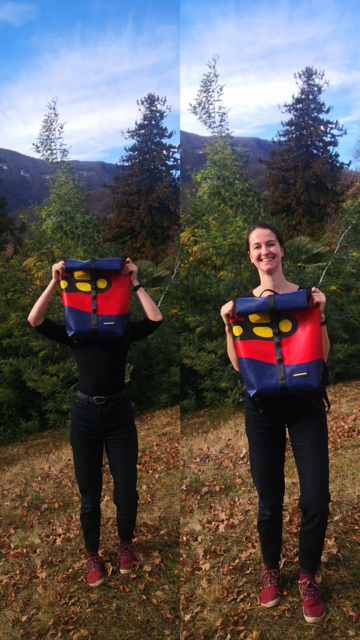
\includegraphics[width=0.3\textwidth]{Tanja}
\caption{The winner of the poster presentations and the poster price - Tanja Holstein Federal Institute of Materials Research and Testing (BAM), Germany; now with the VIB. source: \url{https://twitter.com/HolsteinTanja/status/1616410121600483328}.}
\label{fig:poster}
\end{figure}

\section{Conclusion and outlook}
The EuBIC-MS Developers Meeting 2023 follows the successful previous winter schools and developers meetings.

In a follow-up survey, 50\% of the participants expressed their overall satisfaction with the meeting, with two-thirds of the survey respondents giving it a perfect score (5) and one-third a good score (4).
Overall, opinions varied, with a significant portion favoring either more leisure time or more organized activities, while a notable percentage found the existing balance to be satisfactory.
    
The EuBIC developer's meeting, spanning a few days, witnessed substantial progress across all hackathon sessions, showcasing participants' impressive productivity and teamwork. The commitment of hackathon groups to ongoing collaboration and project completion holds promise for future scientific publications and improved computational mass spectrometric solutions to support proteomics and metabolomics.

Encouraged by the community’s enthusiastic support, the next EuBIC-MS Developers Meeting is scheduled to take place in January 2025.
 
\section{Conflict of interest}
The authors declare no conflict of interest.
 
\section{Acknowledgements}
Sponsoring for the EuBIC-MS 2023 Developers Meeting was provided by \href{https://www.matrixscience.com/}{Matrix Science}, \href{https://www.msaid.de/}{MSAID} and \href{https://biognosys.com/}{Biognosys AG}. The poster price was sponsored by the \href{https://fgcz.ch}{Functional Genomics Center Zurich} of ETH Zurich and University of Zurich. The organization was supported by Congressi Stefano Franscini on Monte Verità, Switzerland. We would like to thank EuPA for their continuing support. We would like to thank all EuBIC-MS members who volunteered to help on all fronts, as well as all keynote speakers, hackathon organizers, and participants who contributed to the success of the Developers Meeting.



%\bibliographystyle{unsrt}
%\bibliographystyle{unsrtnat}
\bibliographystyle{plainnat}
\bibliography{main, github}

%\newpage
%\appendix
%\section{Author affiliation}
\begin{table*}[ht]
\centering
\label{tab:affiliation}

  \resizebox{\textwidth}{!}{
    \begin{tabular}{ll}
    Anna Klimovskaia Susmelj	&	Biognosys, Schlieren, Zurich 8952, Switzerland, now AI Center ETH Zürich\\
Ludwig Lautenbacher	&	Computational Mass Spectrometry, TUM School of Life Sciences, Technical University of Munich, Maximus-von-Imhof-Forum 3, D - 85354 Freising, Germany\\
Mathias Wilhelm	&	Computational Mass Spectrometry, TUM School of Life Sciences, Technical University of Munich, Maximus-von-Imhof-Forum 3, D - 85354 Freising, Germany\\
Veit Schwämmle	&	Department of Biochemistry and Molecular Biology, University of Southern Denmark, Campusvej 55, 5230 Odense, Denmark\\
Pedro Beltrao	&	Department of Biology, ETH Zurich, Switzerland\\
Jonas Scheid	&	Department of Peptide-based Immunotherapy, Institute of Immunology, University and University hospital Tübingen\\
		& Auf der Morgenstelle 15, D-72076 Tübingen, Germany\\
		& Quantitative Biology Center (QBiC), University of Tübingen, Auf der Morgenstelle 10, D-72076 Tübingen, Germany\\
Alexey Nesvizhskii	&	Departments of Pathology and Computational Medicine and Bioinfoirmatics, University of Michigan, Ann Arbor, Michigan, 48105 USA \\
Ralph Schlapbach	&	Functional Genomics Center Zürich, ETH Zurich/University of Zurich, Winterthurerstrasse 190, CH-8057 Zürich, Switzerland\\
Tobias Kockmann	&	Functional Genomics Center Zürich, ETH Zurich/University of Zurich, Winterthurerstrasse 190, CH-8057 Zürich, Switzerland\\
Christian Panse	&	Functional Genomics Center Zürich, ETH Zurich/University of Zurich, Winterthurerstrasse 190, CH-8057 Zürich, Switzerland\\
		&Swiss Institute of Bioinformatics, Quartier Sorge - Batiment Amphipole, 1015 Lausanne, Switzerland\\
Witold E. Wolski	&	Functional Genomics Center Zürich, ETH Zurich/University of Zurich, Winterthurerstrasse 190, CH-8057 Zürich, Switzerland\\
		&Swiss Institute of Bioinformatics, Quartier Sorge - Batiment Amphipole, 1015 Lausanne, Switzerland\\
Matthias Mattanovich	&	Novo Nordisk Foundation Center for Basic Metabolic Research, University of Copenhagen, Blegdamsvej 3B, DK-2200 Copenhagen, Denmark\\
Muyao Xi	&	Novo Nordisk Foundation Center for Basic Metabolic Research, University of Copenhagen, Blegdamsvej 3B, DK-2200 Copenhagen, Denmark\\
Henry Webel	&	Novo Nordisk Foundation Center for Protein Research, Faculty of Health and Medical Sciences, University of Copenhagen, Copenhagen, Denmark\\
Bart Van Puyvelde	&	ProGenTomics, Laboratory of Pharmaceutical Biotechnology, Ghent University, Ottergemsesteenweg 460, BE-9000 Ghent, Belgium\\
Maximilian Strauss	&	Proteomics Program, Novo Nordisk Foundation Center for Protein Research, Faculty of Health and Medical Sciences, University of Copenhagen, Copenhagen, Denmark\\
Dirk Winkelhardt	&	Ruhr-Universität Bochum, Germany\\
Matthew The	&	TUM School of Life Sciences Technische Universität München D - 85354 Freising\\
Alireza Nameni	&	VIB-UGent Center for Medical Biotechnology, 9052, Zwijnaarde, Belgium\\
		& Department of Biomolecular Medicine, Ghent University, 9000, Ghent, Belgium\\
Ralf Gabriels	&	VIB-UGent Center for Medical Biotechnology, 9052, Zwijnaarde, Belgium\\
		& Department of Biomolecular Medicine, Ghent University, 9000, Ghent, Belgium\\
Tanja Holstein	&	VIB-UGent Center for Medical Biotechnology, 9052, Zwijnaarde, Belgium\\
		& Department of Biomolecular Medicine, Ghent University, 9000, Ghent, Belgium\\
Tim Van Den Bossch	&	VIB-UGent Center for Medical Biotechnology, 9052, Zwijnaarde, Belgium\\
		& Department of Biomolecular Medicine, Ghent University, 9000, Ghent, Belgium\\

    \end{tabular}
  }
\caption{Author affiliation; grouped and ordered by affiliation.}
\end{table*}


\end{document}
